\documentclass[border=6pt]{standalone}
\usepackage[T1]{fontenc}
\usepackage{lmodern}
\usepackage{tikz}
\usetikzlibrary{arrows.meta,positioning,shapes.geometric,calc,fit}
\begin{document}
\hyphenpenalty=10000 \exhyphenpenalty=10000
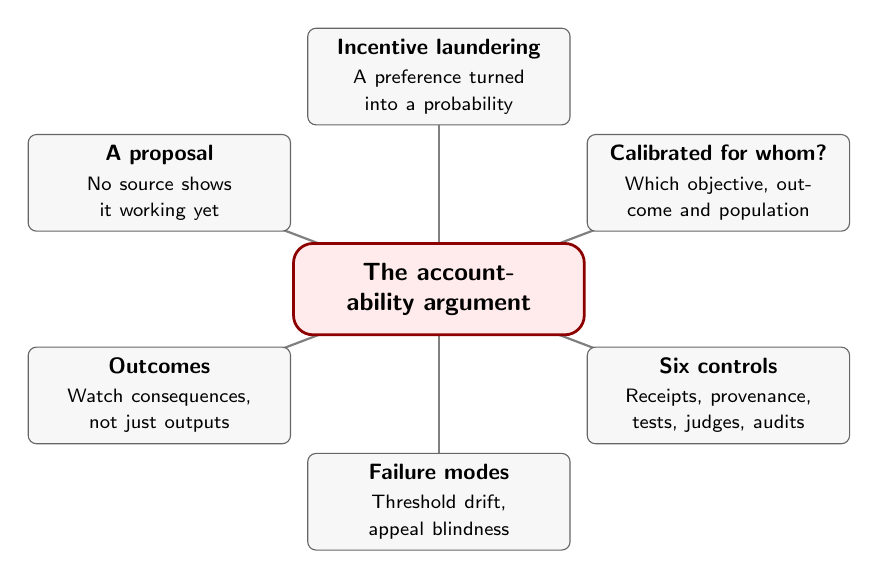
\begin{tikzpicture}[
  font=\footnotesize\sffamily,
  hub/.style={draw=red!55!black, line width=1pt, rounded corners=7pt, fill=red!8, align=center,
              text width=3.2cm, inner sep=7pt, font=\bfseries\small\sffamily},
  br/.style={draw=black!60, rounded corners=3pt, fill=black!3, align=center,
             text width=3.05cm, inner sep=4pt},
  edge/.style={draw=black!50, line width=0.8pt}
]
\draw[edge] (0,0) -- (0.00,2.70);
\draw[edge] (0,0) -- (3.55,1.35);
\draw[edge] (0,0) -- (3.55,-1.35);
\draw[edge] (0,0) -- (0.00,-2.70);
\draw[edge] (0,0) -- (-3.55,-1.35);
\draw[edge] (0,0) -- (-3.55,1.35);
\node[hub] at (0,0) {The accountability argument};
\node[br] at (0.00,2.70) {\textbf{Incentive laundering}\\[1pt]{\scriptsize A preference turned into a probability}};
\node[br] at (3.55,1.35) {\textbf{Calibrated for whom?}\\[1pt]{\scriptsize Which objective, outcome and population}};
\node[br] at (3.55,-1.35) {\textbf{Six controls}\\[1pt]{\scriptsize Receipts, provenance, tests, judges, audits}};
\node[br] at (0.00,-2.70) {\textbf{Failure modes}\\[1pt]{\scriptsize Threshold drift, appeal blindness}};
\node[br] at (-3.55,-1.35) {\textbf{Outcomes}\\[1pt]{\scriptsize Watch consequences, not just outputs}};
\node[br] at (-3.55,1.35) {\textbf{A proposal}\\[1pt]{\scriptsize No source shows it working yet}};
\end{tikzpicture}
\end{document}
